%%%%%%%%%%%%%%%%%%%%%%%%%%%%%%%%%%%%%%%%%%%%%%%%%%%%%%%%%%%%%%%%%%%%%%%%%%%%%
% Chapter 1: Introducci�n 
%%%%%%%%%%%%%%%%%%%%%%%%%%%%%%%%%%%%%%%%%%%%%%%%%%%%%%%%%%%%%%%%%%%%%%%%%%%%%%%

%---------------------------------------------------------------------------------
\section{Antecedentes y estado actual del tema}
\label{1:sec:1}

La World Wide Web esta sujeta a un cambio continuo. La llegada de HTML5, la creciente importancia de AJAX y de la 
programaci\'on en el lado del cliente, las nuevas fronteras de la Web Sem\'antica, la explosi\'on de las redes 
sociales as\'{\i} como la llegada de las redes sociales federadas son ejemplos de esta tendencia general. 
Las aplicaciones web parecen evolucionar hacia entornos cada vez m\'as ricos y flexibles en los que los usuarios 
pueden acceder con facilidad a los documentos, publicar contenido, escuchar m\'usica, ver v\'{\i}deos, realizar dibujos
e incluso jugar usando un navegador. Esta nueva clase de software ubicuo no cesa de ganar \textit{momentum} y promueve nuevas 
formas de interacci\'on y cooperaci\'on.
\bigskip

Dentro del \'ambito educativo tambi\'en se ha vivido una revoluci\'on, en forma y contenido, de impartir ense�anza.
En Internet se puede encontrar, cada vez con m\'as facilidad, contenidos de cualquier disciplina en m\'ultiples
formatos: blogs, videotutoriales, presentaciones, ejercicios resueltos, etc.

Tambi\'en est\'an teniendo mucho \'exito las plataformas de aprendizaje virtual ofreciendo, adem\'as de conocimiento 
sin la necesidad de estar f\'{\i}sicamente presente en un aula, una serie de recompensas y medallas por ir obteniendo
logros. Esta metodolog\'{\i}a se denomina {\bfseries Gamificaci\'on} y est\'a teniendo un impacto muy positivo en los usuarios
de estas plataformas, ya que los anima a seguir usando estas herramientas de conocimiento.
\bigskip

Otro tipo de plataforma de aprendizaje virtual m\'as orientada a universidades e institutos es {\bfseries Moodle}. Est\'a implamantada
en numerosos centros de todo el planeta. Es el complemento perfecto para enriquecer las ense�anzas impartidas f\'{\i}sicamente
con cuestionarios autoevaluativos y compartici\'on de recursos adicionales. Adem\'as, facilita numerosas tareas a los docentes como 
la correcci\'on y calificaci\'on de ejercicios.

Sin embargo, esta plataforma s\'olo se limita a la evaluaci\'on de cuestiones triviales. Para la correci\'on de preguntas
propias de las ramas de Ingenier\'{\i}a, como pueden ser la implementaci\'on de c\'odigo, es necesaria la figura del profesor para
evaluar dichas tareas.

Otro problema que presenta es su dif\'{\i}cil portabilidad. Estamos hablando de un tipo de plataforma que sigue un
esquema {\bfseries cliente-servidor}, que no es f\'acilmente migrable a otras m\'aquinas.
\bigskip

Estas desventajas se ven resueltas con la {\bfseries Aplicaci\'on para la Elaboraci\'on y Despliegue de Cuestionarios} que se presentar\'a
en esta memoria.

%---------------------------------------------------------------------------------
\section{�Qu\'e es RuQL?}
\label{1:sec:2}

Esta aplicaci\'on de generaci\'on y despliegue de cuestionarios forma parte de una
gema de Ruby creada por \href{http://www.armandofox.com/geek}{Armando Fox} denominada 
\href{http://github.com/saasbook/ruql}{'Ruby-based Quiz Generator and DSL'} (RuQL).

Inicialmente, esta gema permit\'{\i}a generar un cuestionario partiendo de un fichero {\bfseries Ruby}, 
donde se redactaban las preguntas y respuestas haciendo uso de un {\bfseries DSL}.

Pose\'{\i}a una serie de \textit{renderers} que permit\'{\i}an generar los cuestionario en los siguientes formatos:
\begin{itemize}
  \item \href{http://code.edx.org/}{Open EdX}: formato \textit{open source} listo para importar en plataformas de aprendizaje online como {\bfseries EdX}.
  \item Versi\'on HTML 5 imprimible: lista para ser impresa y rellenada por los usuarios.
  Se le pod\'{\i}a pasar como argumento el path de una hoja de estilo para incorporarla al HTML de salida. Del mismo modo, se
  pod\'{\i}a especificar el path de un template predefinido por el profesor de modo que las preguntas se renderizaran en el mismo.
  \item \href{http://home.gna.org/auto-qcm}{AutoQCM}: formato listo para importar a {\bfseries AMC} (\textit{Auto Multiple Choice}), software libre
  que permite elaborar cuestionarios multirrespuesta.
\end{itemize}

Los tipos de preguntas que se pod\'{\i}an especificar eran:
\begin{itemize}
  \item {\bfseries Preguntas de completar}: en las cuales los usuarios deben rellenar los espacios en blanco. Admit\'{\i}a respuestas de tipo \textit{string} o
  \textit{regexp}. Si exist\'{\i}an m\'ultiples espacios para rellenar, se especificaban las respuestas en forma de \textit{array}, indicando adem\'as
  si el orden de las mismas influ\'{\i}a.
  Permit\'{\i}a adem\'as especificar respuestas falsas (\textit{distractors}) con una explicaci\'on de la misma, de modo que si el 
  alumno escrib\'{\i}a dicho \textit{distractor}, le apareciera la explicaci\'on de por qu\'e esa respuesta era incorrecta.
  
  [foto]
  
  \item {\bfseries Preguntas multirrespuesta con una  \'unica respuesta correcta}: las cl\'asicas preguntas tipo test. Se pod\'{\i}a aleatorizar el orden
  de las respuestas definido en el fichero de preguntas y asignarles explicaciones a los \textit{distractors} de manera individual o asignar una explicaci\'on
  general para todos los \textit{distractors}.
  
  [foto]
  
  Especificando adem\'as la opci\'on \textit{raw} a la pregunta, permit\'{\i}a incrustar dicho texto entre etiquetas \textless pre\textgreater \space HTML.
  
  [foto]
  
  \item {\bfseries Preguntas multirrespuesta con una  m\'ultiples respuestas correctas}: iguales a las preguntas multirrespuesta de opci\'on \'unica con la diferencia de 
  que existe m\'as de una respuesta correcta.
  
  [foto]
  
  \item {\bfseries Preguntas de verdadero o falso}: caso particular de las preguntas multirrespuesta de opci\'on \'unica.
  
  [foto]
  
\end{itemize}

Para todos los tipos de preguntas era posible especificar un comentario opcional que acompa�ar\'{\i}a al texto de la pregunta.

%---------------------------------------------------------------------------------
\section{Objetivos y actividades a realizar}
\label{1:sec:3}

Los objetivos propuestos para alcanzar en este Trabajo de Fin de Grado ha sido los siguientes:
\begin{itemize}
  \item Conocer, dominar y practicar con lenguajes y herramientas de desarrollo de aplicaciones web en el {\bfseries servidor}.
  \item Conocer, dominar y practicar con diferentes lenguajes y librer\'{\i}as en el {\bfseries cliente}.
  \item Conocer, practicar y dominar de herramientas de {\bfseries desarrollo dirigido por pruebas} (\textit{TDD}) en entornos web.
  \item Conocer, practicar y dominar diferentes lenguajes de marcas y de estilo.
  \item Conocer, practicar y dominar diferentes mecanismos de despliegue.
  \item Conocer, practicar y familiarizarse con diferentes mecanismos de seguridad, autentificaci\'on y autorizaci\'on.
  \item Conocer, practicar y dominar diferentes herramientas colaborativas y de {\bfseries control de versiones} (\textit{CVS}).
  \item Conocer, practicar y dominar {\bfseries metodolog\'{\i}as \'agiles} de desarrollo de software.
  \item Desarrollar una aplicaci\'on web para la elaboraci\'on y despliegue de cuestionarios.
\end{itemize}
\bigskip

Y las actividades a realizar en el mismo, tal cual est\'an descritas en la propuesta de {\bfseries Proyecto de Trabajo de Fin de Grado} firmada por 
el director y el alumno en la actividad 2 de la asignatura, son las que se describen a continuaci\'on:
\begin{itemize}
  \item Revisi\'on bibliogr\'afica.
  \item Realizaci\'on de una aplicaci\'on web en la que:
  \begin{itemize}
    \item Se proporciona soporte mediante una aplicaci\'on web a los procesos de evaluaci\'on.
    \item Se proporciona/extiende un {\bfseries Lenguaje de Dominio Espec\'{\i}fico} (\textit{DSL}) para la elaboraci\'on de cuestionarios.
    \item Se deber\'a considerar c\'omo resolver los problemas de seguridad asociados.
    \item Redacci\'on de la memoria.
  \end{itemize}
  \item Preparaci\'on de las presentaciones.
\end{itemize}



%---------------------------------------------------------------------------------
\section{Tecnolog\'{\i}a usada}
\label{1:sec:4}

Debido a que este Trabajo de Fin de Grado es una extensi\'on de una gema de {\bfseries Ruby}, se ha utilizado \'este como lenguaje de
programaci\'on.

Adem\'as, se ha hecho uso de un numeroso conjunto de gemas y de otras tecnolog\'{\i}as enumeradas a continuaci\'on:
\begin{itemize}
  \item HTML5: haciendo uso de funcionalidades como {\bfseries Local Storage} y {\bfseries Drag and Drop}.
  \item CSS3
  \item JavaScript
  \item \href{http://getbootstrap.com/}{Bootstrap}
  \item \href{https://jquery.com/}{jQuery}
  \item \href{http://xregexp.com/}{XRegExp}
  \item \href{http://www.mathjax.org/}{MathJax}
  \item \href{http://codemirror.net/}{CodeMirror}
  \item \href{https://visionmedia.github.io/mocha/}{Mocha}
  \item \href{http://chaijs.com/}{Chai}
  \item \href{https://karma-runner.github.io/0.12/index.html}{Karma}
  \item \href{http://www.sinatrarb.com/}{Sinatra}
  \item \href{https://github.com}{GitHub}
  \item \href{https://www.heroku.com/}{Heroku}
  \item \href{http://oauth.net/2/}{OAuth 2.0}
  \item \href{https://drive.google.com}{Google Drive}
  
  \bigskip
  [Iconos]
\end{itemize}


%------------------------------------------------------------------------------
\begin{figure}[!th]
\begin{center}
\includegraphics[width=0.5\textwidth]{images/arbolbinario.eps}
\caption{Ejemplo}
\label{fig:ArbolBinario}
\end{center}
\end{figure}
%------------------------------------------------------------------------------

